%
% Modified by Sameer Vijay
% Last Change: Wed Jul 27 2005 13:00 CEST
%
%%%%%%%%%%%%%%%%%%%%%%%%%%%%%%%%%%%%%%%%%%%%%%%%%%%%%%%%%%%%%%%%%%%%%%%%
%
% Sample Notre Dame Thesis/Dissertation
% Using Donald Peterson's ndthesis classfile
%
% Written by Jeff Squyres and Don Peterson
%
% Provided by the Information Technology Committee of
%   the Graduate Student Union
%   http://www.gsu.nd.edu/
%
% Nothing in this document is serious except the format.  :-)
%
% If you have any suggestions, comments, questions, please send e-mail
% to: ndthesis@gsu.nd.edu
%
%%%%%%%%%%%%%%%%%%%%%%%%%%%%%%%%%%%%%%%%%%%%%%%%%%%%%%%%%%%%%%%%%%%%%%%%

%
% Chapter 4
%

\chapter{DATA ANALYSIS}
\label{chap:dataAnalysis}
Show 74,76Ge data obtained
Show extracted cross section for 0+ ground state (show other states?)

error calculations: its own section?

\section{Extracting Absolute Cross Sections}
detector efficiency (this will take an entire section/subsection)
beam current
target thickness, RBS measurements, alpha measurements
dead time
SOLID ANGLE!

go ahead and discuss errors while you discuss these quantities

two data sets
- pulse selection
- no pulse selection

background
- gamma peaks - do not overlap with neutron peak
- other neutron peaks - ??
- randoms - background in both data sets
- continuum - more important in non-pulse-selected data

extracting counts 
- pulse selection
- no pulse selection

The data sets for this analysis were gathered in two seperate runs; the pulse selector was not working for part of the first run.  Analysis of the datasets taken with pulse selection is straigtforward and will be discussed first.  Without pulse selection, the neutron peak sits on top of background from previous neutron bunches.  The background fit is different and the total counts have a larger systematic uncertainty; extracting these will be discussed second.

\subsection{Error Analysis - Counts}
In the TOF spectrum, the neutron peak sits on top of random background and also beam-induced background.  If the background is well-known, extracting the counts due to the neutrons is simple:

Sum(peak region) - Background(peak region)

The error associated with this quantity is [ref?]

$sqrt(\sigma_Sum^2 + \sigma_background^2)$

The number of counts in the peak region are a sum of the number of counts in the random background and counts from the neutrons.  The width of a sample at a uniform rate is simply sqrt(N), as seen in figure ??.  This is an appropriate description of the random background.  The neutron peak is roughly gaussian-shaped, and running trials where counts are drawn from a gaussian distribution shows that the width is ??.

Thus $\sigma_{Sum}$ is approximately $sqrt(N_{peakregion})$.

\begin{figure}[ht]
\centering
  \subfloat[Distribution of Background Counts][Distribution of Background Counts]{
  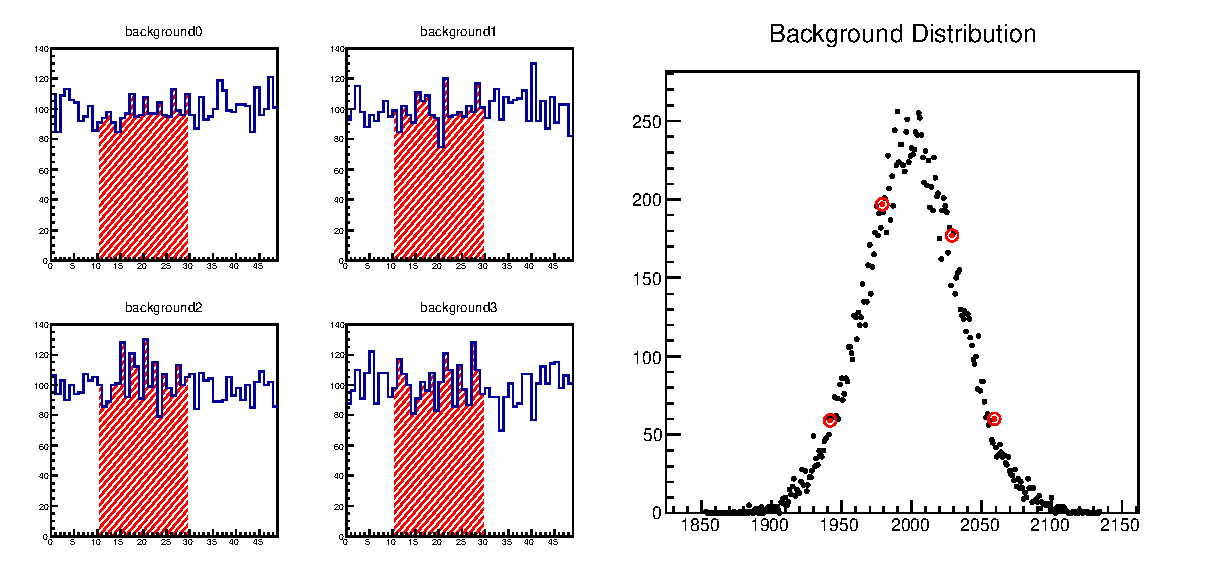
\includegraphics[width=0.9\textwidth]{figures/bkgDist}
  \label{fig:bkgDist}}
  
  \subfloat[Distribution of Signal Counts][Distribution of Signal Counts]{
  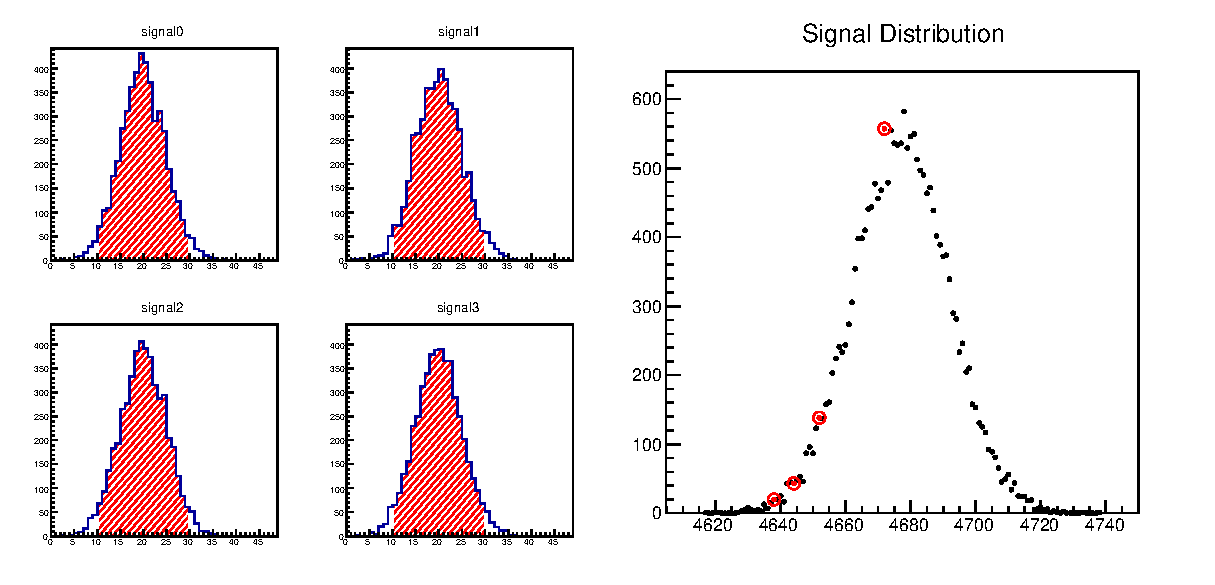
\includegraphics[width=0.9\textwidth]{figures/sigDist}
  \label{fig:sigDist}}
  
  \subfloat[Distribution of Extracted Counts][Distribution of Extracted Counts]{
  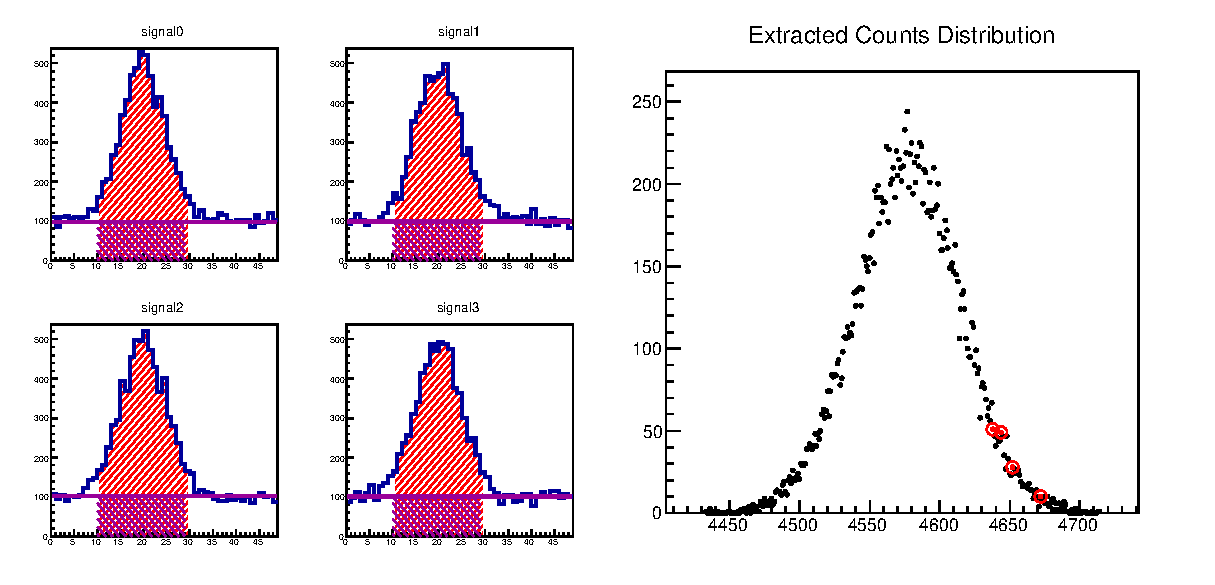
\includegraphics[width=0.9\textwidth]{figures/extractDist}
  \label{fig:extractDist}}

  \caption{This is a figure containing several subfigures.}
  \label{fig:statDist}
\end{figure}

The error associated with the background depends on how the background is determined.  In most cases, the background is fit.  When the background is fit, the error associated with the number of counts is the error associated with the fit parameters when propagated through the appropriate integral.  For the pulse-selected data, the fit is to a constant and contributes less than a tenth of a percent to the total error.  The non-pulse-selected data does not enjoy such an ambiguous fit and contributes approximately ??\% to the total error.

\subsection{Pulse-Selected Data}
With pulse selection, the region behind the neutron peak has only random signal and can be fit with a constant to within ??\%.  Assuming that the neutron peak itself does not overlap with other background, the total number of counts is estimated as the direct sum of the bin contents minus the average bin content of the background region.  In this case, the error should be the statistical error associated with the random background in the peak region and the statistical error associated with the counts in the neutron peak, added in quadrature.  Such an error neglets the error associated with the constant that is fit, appropriate in this case because it influences the error by at most 0.1\%.

When considering the error, it should be considered that the neutron peak itself may be sitting on top of signal from processes that result in lower-energy neutrons.  A neutron continuum is clearly visible in all targets, and while in 26Mg the continuum is separated by ?? MeV, it is difficult to determine where the continuum for the 76Se and 78Se stops.  What is safe to assume is that neutrons populating the continuum cannot have an energy greater than the 0+ neutron, and so its endpoint cannot extend past the center of the ground state neutron distribution.  Functional models that fit the shape of the continuum well are the Beta Distribution and also the Gamma Distribution.  Both these functions give similar estimates of the background under the neutron peak; the effect is not greater than ??\% even in the largest peaks.

\subsection{Data with No Pulse Selection}
With no pulse selection, the neutron peak sits on top of background from the previous bunch.  Not surprisingly, the sensitivity to the fit to the continuum is larger - as much as ??\% in some cases.

\section{Placing a limit on excited 0+ state cross-sections}
introduce 0+ peak and see when it becomes statistically significant
there will be different limits for different energies!  because of the evaporation background

\section{Fitting 0+ ground state}
DWBA calculation
shell model
f$^2$, p$^2$ state strength ("form factor")

\section{Implications for \zvbb NME}
Okay I'm not really sure how to figure this out

% % uncomment the following lines,
% if using chapter-wise bibliography
%
% \bibliographystyle{ndnatbib}
% \bibliography{example}
